\documentclass[acmtog]{acmart}
\usepackage{graphicx}
\usepackage{subfigure}
% Title portion
\title{Assignment 1 : Creating your own OpenGL program} 
\author{Name:\quad Zhang Zhanrui  \\ student number:\quad 2019533227
	\\email:\quad zhangzhr2@shanghaitech.edu.cn}

% Document starts
\begin{document}
\maketitle

\vspace*{2 ex}

\section{Introduction}

In this Assignment, the following tasks are finished. First, the mesh object in resources folder are loaded. Then they are properly drawn on the screen. After that, multiple lighting was added to the object, based on the Phong shading model. At last, keyboard and mouse input are handled so that we can move around in the scene and watch those objects all directions.

\section{Implementation Details}

\subsection{Loading Meshes From File}

First we need to load the mesh file into our program. To make it clear, this part is implement in the `.scr/loadmesh.h' file. Given the file name, then the object is load into a `Mesh' class, which contains 4 members. 
\begin{itemize}
	\item 
	`vertexAttrib' is a float vector. It contains all the vertex attribute. In our cases, it is three number representing vertex position and then three number representing normal direction.
	\item	
	`indices' is a integer vector. It contains the indices of vertices of each triangle. The index starts from 0.
	\item	
	`v\_num' and `f\_num' are two integers that record the number of vertices and faces of the obj.
\end{itemize}

In `main.cpp', I created two `Mesh' objects called Bunny and Pumpkin, now we can send these data into the rendering pipeline.

\subsection{Draw Meshes on the screen}
Once loading the meshes and store them in vectors, we can draw them on the screen.


\subsubsection{Bound Vertex Attribute}
We need to create a VBO object and bind the vector containing vertex attribute onto it. We need to create EBO and do similar things for index vector. At last we bind VBO and EBO on VAO. Two VAO are created to handle two objects.


\subsubsection{Shader Program}
After binding those vertex attribute, two more shader programs are needed in the rendering pipeline -- vertex shader and fragment shader. We are provided with a shader class. We only need to provide the path to our shader program, and it will create, compile the shader for us.

\subsubsection{Vertex Shader}
The vertex shader receives data from VBO object. First, `layout' is used to tell the shader where each vertex attribute is. In out cases, we have two vertex attributes -- vertex position and normal.

For vertex position, The input position from VBO is local space, while the output should be the coordinate in clip space, which is a cube. so we need to apply three matrix.

The model matrix transform the coordinate into the world space. This matrix is manually implemented. For bunny, I keep it in origin with model matrix being identical matrix. For pumpkin, I moved it a little bit.

The view matrix transform the coordinate into view space. For bunny and pumpkin, this transformation is the same. The view matrix is kept in `camera' class in `main.cpp'.

The projection matrix project the object in the frustum into a cube. This matrix is also the same for bunny and pumpkin. This matrix can be created by using the `perspective()' function provided by glm.

All three matrix above can be created in `main.cpp' and pass to the shader by using `uniform'. A variable with keyword `uniform' is required in the shader program. In `main.cpp', we just need to call `setMat4( )' in `shader.h' provided by TA.

At last, these matrices are applied to vertex position and the result is assigned to `gl\_Position'.


\subsection{Lighting}
So far, the object we have drawn just have shape but do not have shadow, so we need to add lighting.
Fragment shader controls the behavior of each fragment. The output from the vertex shader will be interpolated automatically.


\subsubsection{Multiple Light Sources}
As is required, I placed 2 light sources in my scene. To define a point light source, we need its position in the world space and its color. I set coordinate of light in world space in main function and pass it into the shader by setting two uniform variable in vertex shader. The lighting calculation will be performed in view space, so view transformation is needed. We just apply view matrix on light position and pass the results into the fragment shader.


\subsubsection{Ambient Light}
Ambient light comes from the reflection of environment. Here I assume that the environment is white, which means the reflection color is just the same as the color of light source. Then I just need to define a `ambt\_factor' to represent the strength of ambient light.


\subsubsection{Diffuse Light}
Diffuse light depends on the relationship between light source and object.

We already have the light source position in view space in fragment shader.

To know the position and normal of object in view space, we just need to apply corresponding transformation matrix on their position to get the coordinate in view space and output them to fragment shader.

Now, we have everything in the view space, just calculate dot product of light direction and normal vector to figure out how strong the diffuse color will be.

\subsubsection{Specular Light}
When calculating diffuse light, we already have the light direction and normal in view space. We can use reflect function to calculate the reflection and compare it to the `view vector' which is easy to calculate since the camera is on origin and reflection point is known. 


After knowing how strong ambient, diffuse and specular light is, we just add them together, then times the color of light source, we can get the color of the fragment. Since there are two light source in the scene, we need to add two color together to get the final output color.

\subsection{Camera control}

I defined an FPS style camera in this assignment. The goal is to control the camera in the following manner:
\begin{itemize}
	\item move the camera up and down along the up direction of camera by pressing `W' and `S'.
	\item move the camera left or right along the right direction of camera by pressing `A' and `D'.
	\item move the camera forward and backward along the gaze direction of camera by pressing `R' and `F'.
	\item pitch and yaw the camera by mouse.
\end{itemize}

A class `camera' is defined in the file `camera.h'. It contains several members:
\begin{itemize}
	\item a $4\times4$ matrix: this is the view matrix, defining how we transform the world space to the view space.
	\item Three vectors: `camPos', `camGaze', `camUp', defining the camera's position, directions it looking at, and up direction in the world space.
	\item Two doubles: `yaw' and `pitch' to record the pitch and yaw angle of the camera.
\end{itemize}

\subsubsection{Control with keyboard}

The code skeleton has already defined a `processInput' function to handle the ESC input for exiting the program, so similarly I add 6 more conditional branches to handle the input from `A', `S', `D', `W', `R', `F'. Once a key is pressed, we can call corresponding move function to change corresponding vector and them update the view matrix.

\subsubsection{Control with mouse}
To control with mouse, a call back function is needed. And we just calculate the distance the mouse moved on X and Y direction and corresponding shift on variable `yaw' and `pitch', and then update the view matrix.


\subsection{Enable MSAA}
GLFW has provided us with corresponding multi-sample anti-aliasing functionality, we need to call `glfWindowHint( )' and tell glfw the number of sub-sampling point we need. Then we need to call `glEnable(GL\_MULTISAMPLE)' to enable MSAA.

\section{Results}
The results can be seen in the picture. The bunny is placed on the origin, and the pumpkin is moved and scaled down a little bit to avoid intersection. Both object's base color are set to 60\% grey. Two point lights are placed. One brighter, yellow light in the front, and one darker, blue light in the back.



\begin{figure}[h]
\centering
\subfigure[front]
{
	\begin{minipage}[b]{.4\linewidth}
		\centering
		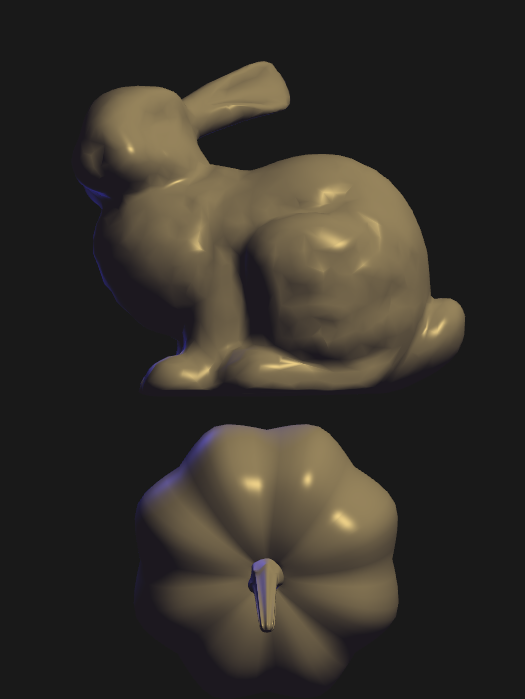
\includegraphics[scale=0.25]{front.png}
	\end{minipage}
}
\subfigure[back]
{
		\begin{minipage}[b]{.4\linewidth}
		\centering
		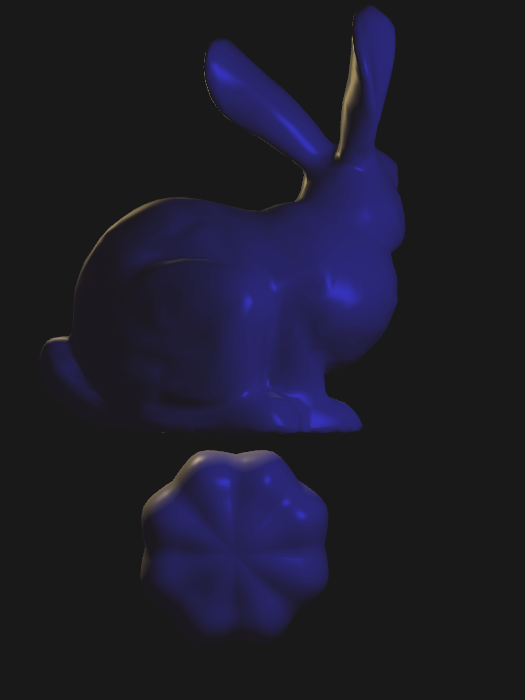
\includegraphics[scale=0.25]{back.png}
	\end{minipage}
}
\\
\subfigure[left] 
{
		\begin{minipage}[b]{.4\linewidth}
		\centering
		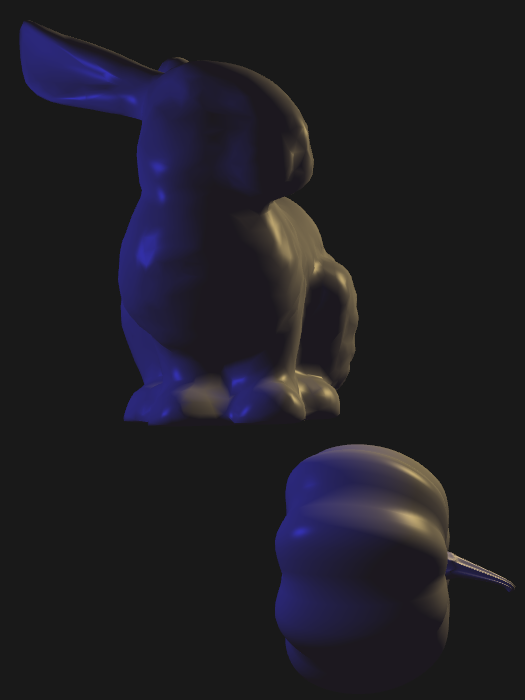
\includegraphics[scale=0.25]{left.png}
	\end{minipage}
}
\subfigure[right]
{
		\begin{minipage}[b]{.4\linewidth}
		\centering
		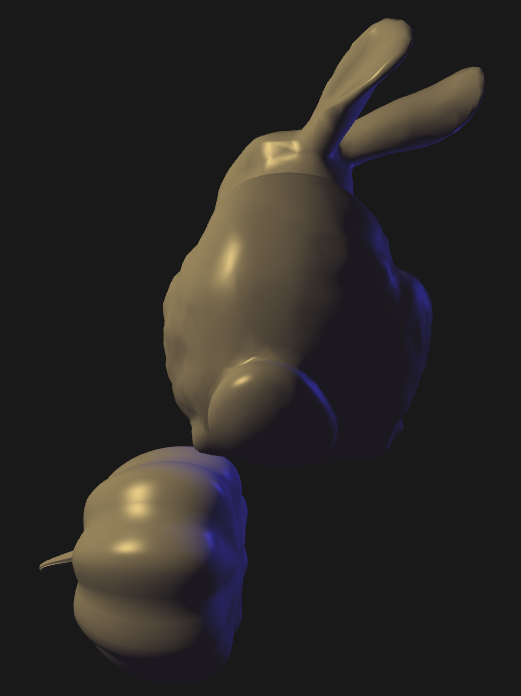
\includegraphics[scale=0.25]{right.png}
	\end{minipage}
}
\caption{different angle}
\end{figure}


Comparing the result before and after enabling MSAA, it is clear that the edge of the object become smooth after enabling MSAA.


\begin{figure}[h]
\centering
\subfigure[MSAA enabled]
{
	\begin{minipage}[b]{.4\linewidth}
		\centering
		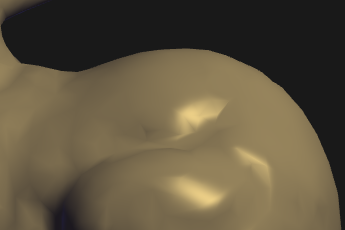
\includegraphics[scale=0.39]{withMSAA.png}
	\end{minipage}
}
\subfigure[MSAA disabled]
{
		\begin{minipage}[b]{.4\linewidth}
		\centering
		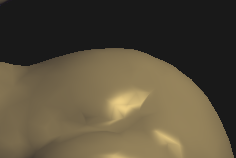
\includegraphics[scale=0.57]{withoutMSAA.png}
	\end{minipage}
}
\caption{Anti-aliasing}
\end{figure}


\end{document}
